% This file was created by matlab2tikz.
%
\definecolor{mycolor1}{rgb}{0.89412,0.10196,0.10980}%
\definecolor{mycolor2}{rgb}{0.21569,0.49412,0.72157}%
%
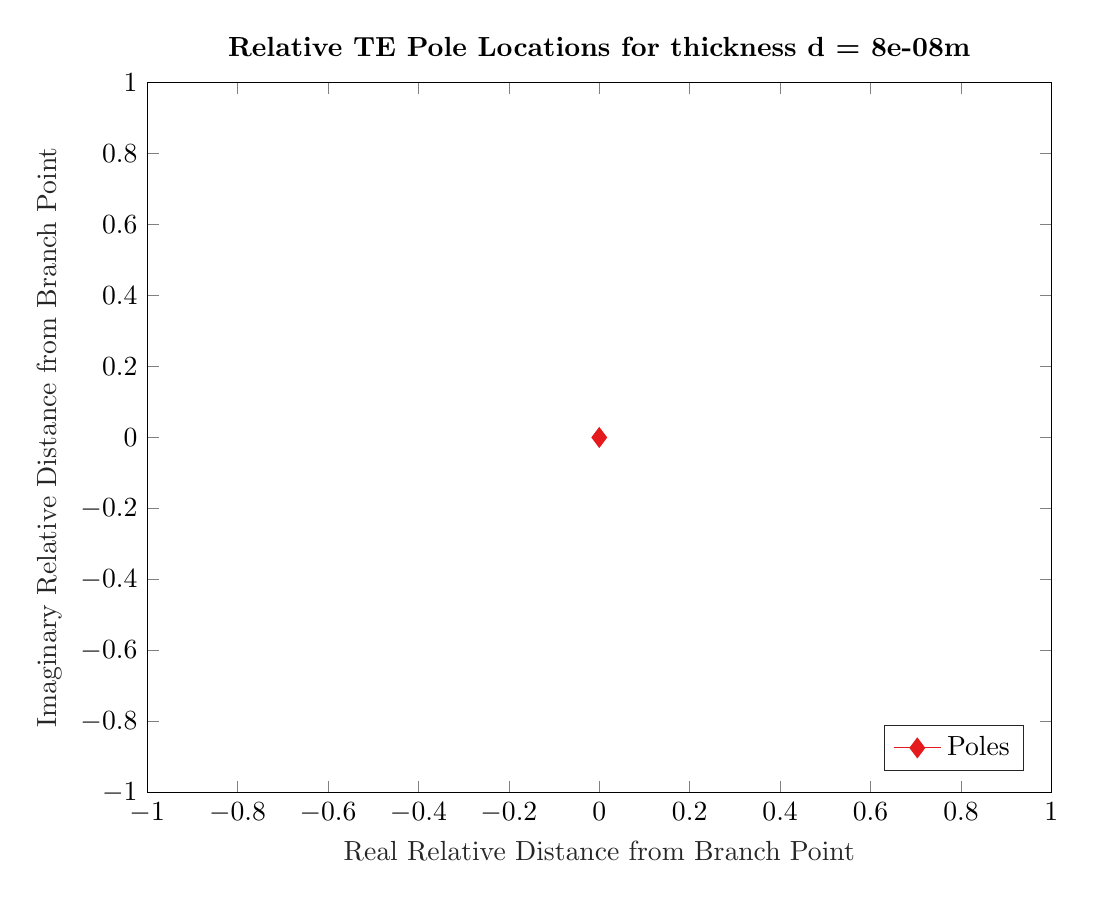
\begin{tikzpicture}

\begin{axis}[%
width=4.521in,
height=3.55in,
at={(0.758in,0.497in)},
scale only axis,
xmin=-1,
xmax=1,
xlabel style={font=\color{white!15!black}},
xlabel={$\textrm{Real Relative Distance from Branch Point}$},
ymin=-1,
ymax=1,
ylabel style={font=\color{white!15!black}},
ylabel={$\textrm{Imaginary Relative Distance from Branch Point}$},
axis background/.style={fill=white},
title style={font=\bfseries},
title={Relative TE Pole Locations for thickness d = 8e-08m},
legend style={at={(0.97,0.03)}, anchor=south east, legend cell align=left, align=left, draw=white!15!black}
]
\addplot [color=mycolor1, draw=none, mark size=3.5pt, mark=diamond*, mark options={solid, fill=mycolor2, mycolor1}]
  table[row sep=crcr]{%
0	0\\
};
\addlegendentry{Poles}

\end{axis}
\end{tikzpicture}%